\documentclass{article}

% Language setting
% Replace `english' with e.g. `spanish' to change the document language
\usepackage[english]{babel}

% Set page size and margins
% Replace `letterpaper' with `a4paper' for UK/EU standard size
\usepackage[letterpaper,top=2cm,bottom=2cm,left=3cm,right=3cm,marginparwidth=1.75cm]{geometry}

% Useful packages
\usepackage{amsmath}
\usepackage{graphicx} % Required for including images
\usepackage{cite}     % Required for handling citations
\usepackage[colorlinks=true, allcolors=blue]{hyperref}

\usepackage{listings}
\usepackage{xcolor}
\usepackage{subcaption}
\usepackage{wrapfig}
\usepackage{float}

% Define colors for syntax highlighting
\definecolor{keywordcolor}{RGB}{0,0,255}
\definecolor{commentcolor}{RGB}{0,128,0}
\definecolor{stringcolor}{RGB}{255,0,0}

% Set the style for C++ code
\lstdefinestyle{cppstyle}{
	language=C++,
	keywordstyle=\color{keywordcolor},
	commentstyle=\color{commentcolor},
	stringstyle=\color{stringcolor},
	basicstyle=\ttfamily,
	numbers=left,
	numberstyle=\tiny,
	stepnumber=1,
	numbersep=5pt,
	frame=single,
	tabsize=4,
	breaklines=true
}

% Define code style
\lstdefinestyle{cppstyle2}{
  language=C++,
  basicstyle=\ttfamily\footnotesize,
  keywordstyle=\color{blue},
  commentstyle=\color{green!50!black},
  stringstyle=\color{red},
  numbers=left,
  numberstyle=\tiny, 
  stepnumber=1,
  breaklines=true,
  backgroundcolor=\color{gray!10},
  frame=single
}


\title{Self Balancing Robot}
\author{Muhammad Haris Mujeeb}

\begin{document}
\maketitle

\begin{abstract}
This report focuses on the design of a Two-wheeled Self-Balancing Robot, which embodies the classic inverted pendulum problem. Using a Kalman filter for MPU6050 sensor data fusion and implementing PID controllers. This project aims to develop a robust two-wheeled self-balancing robot that can be observed and controlled remotely. The coding for the Arduino Nano has been executed using \href{https://platformio.org/}{PlatformIO}, with the complete project available on this \href{https://github.com/haris-mujeeb/Self-Balancing-Robot}{GitHub repository}.
\end{abstract}

\thispagestyle{empty}
\tableofcontents
\listoffigures
\listoftables
\newpage

\section{Introduction}
\subsection{Background \& Motivation}
Two-wheeled vehicles are generally more agile, allowing easier navigation through tight spaces, making them ideal for congested environments. Their lighter weight and compact size facilitate easier handling while also enhancing energy efficiency. In addition, they are typically less expensive to purchase and maintain, increasing accessibility for a wider range of users.
A good base model to build such robot is \href{https://www.elegoo.com/products/elegoo-tumbller-self-balancing-robot-car}{ELEGOO Tumbler} (shown in Fig. 
\ref{fig:tumbler}), which provided nearly all the hardware required as a DIY kit.
\begin{figure}[h]
    \centering
    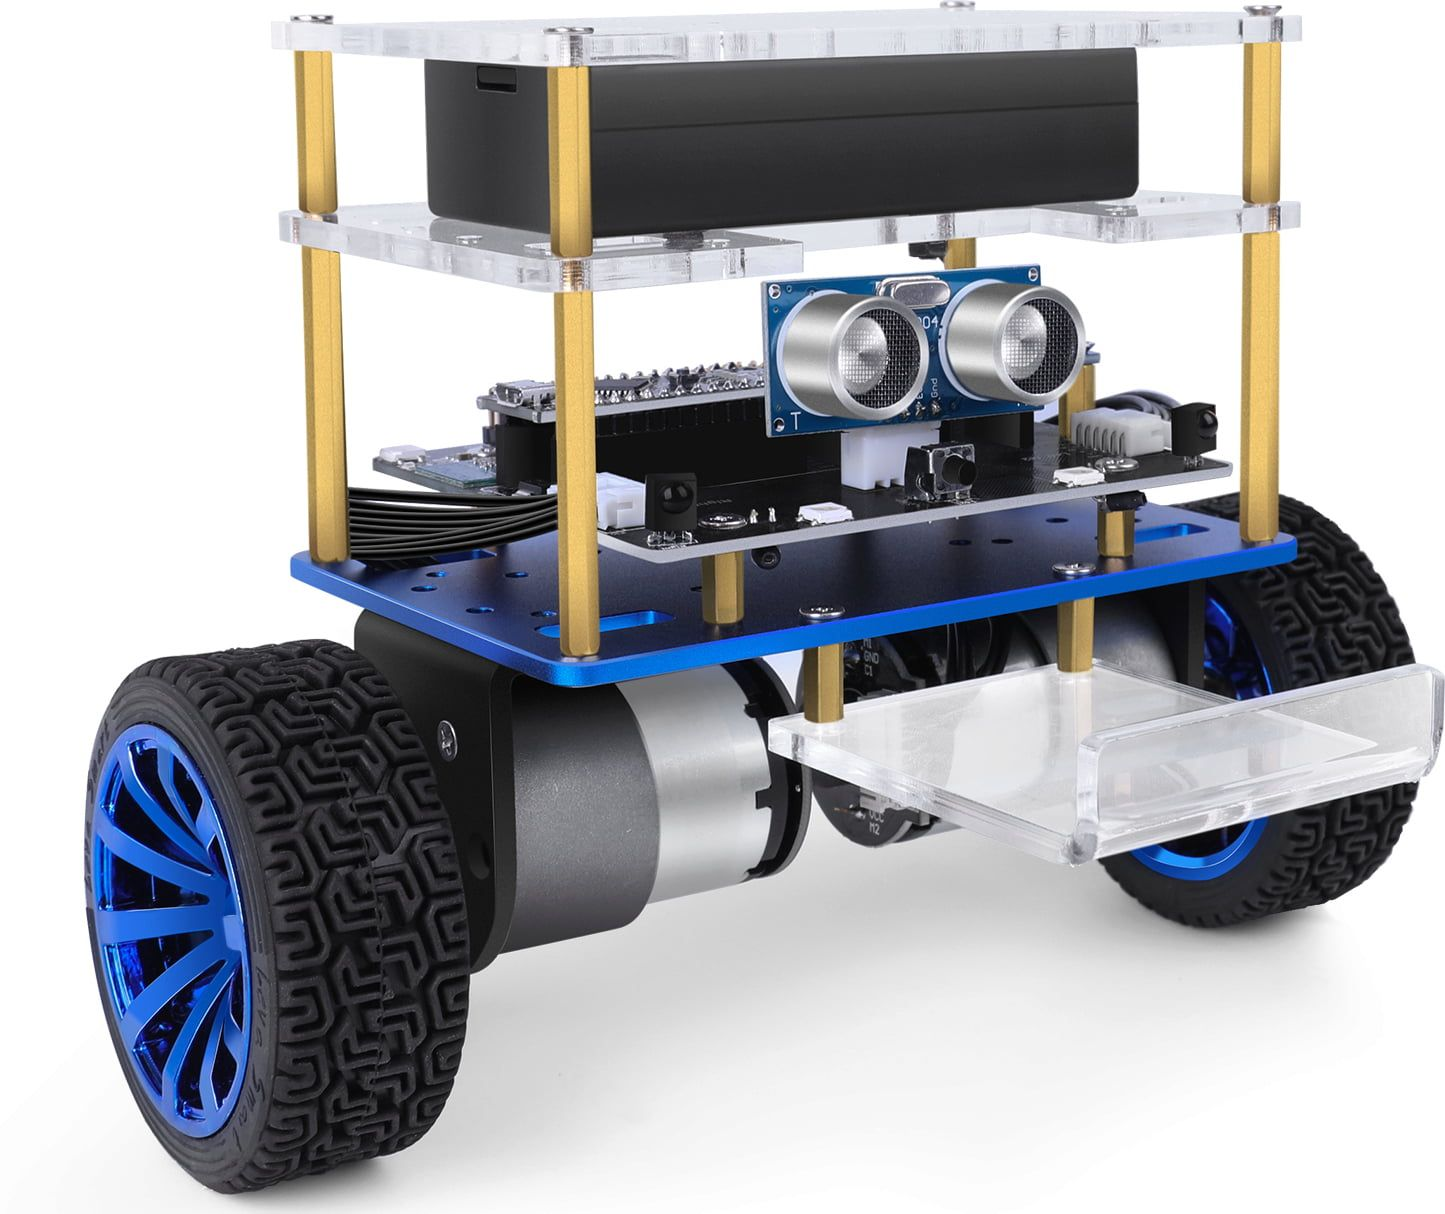
\includegraphics[height=6cm]{assets/tumbler.jpg}
    \caption{\label{fig:tumbler} ELEGOO Tumbler which was used for this project \cite{elegoo}.}
\end{figure}

\subsection{Project Objectives}

\subsection{Scope of Work}


\section{Literature Review}
\subsection{Overall Architecture}
Block diagram of the system
Explanation of the control flow


\subsection{Hardware Components}
\subsubsection{Microcontroller}
The ATmega328P (shown in Fig. \ref{fig:ATmega328p}) is a popular microcontroller from Microchip Technology, widely used in embedded systems and electronics projects. With a 16 MHz clock speed, 32 KB of flash memory, 2 KB of SRAM, and 1 KB of EEPROM \cite{atmega_microchip}, the ATmega328P provides ample resources for this projects application. 

\begin{figure}[h]
	\begin{subfigure}{0.5\textwidth}
	    \centering
		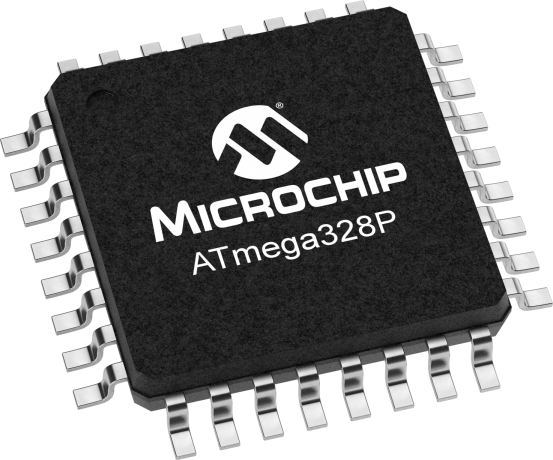
\includegraphics[height=3cm]{assets/ATmega328p.png}
		\caption{ATMEGA328P ANR \cite{atmega_microchip}.}
		\label{fig:ATmega328p}
	\end{subfigure}
	\begin{subfigure}{0.5\textwidth}
    	\centering
		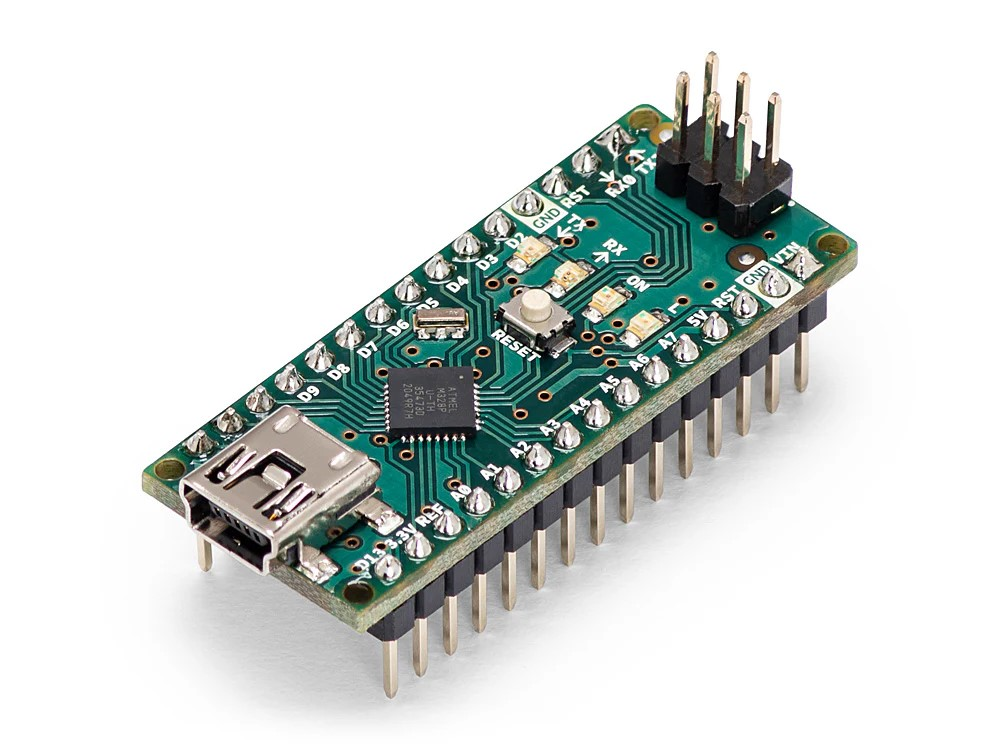
\includegraphics[height=3cm]{assets/arduino_nano.jpg}
		\caption{Arduino Nano \cite{arduino_nano}.}
		\label{fig:arduino_nano}
	\end{subfigure}
	 \caption{ATMEGA328P MCU (a) and Arduino Nano development board (b).} % Caption for the whole figure
	\label{fig:ATmega328p_and_arduino_nano}
\end{figure}

The ATMEGA328P is also used in the Arduino Nano (shown in Fig. \ref{fig:arduino_nano}), a widely adopted development board known for its low cost and open-source ecosystem \cite{arduino_nano}. The combination of affordability and extensive community support makes it an ideal choice for rapid prototyping and academic research, ensuring easy integration with various sensors and motor drivers. 


\subsubsection{Inertial Measuring Unit}
The MPU6050 is a widely used six-axis sensor that integrates a three-axis gyroscope and a three-axis accelerometer on a single chip, making it essential for motion tracking and stabilization applications (shown in Fig. \ref{fig:mpu-6050}). Its compact design and built-in Digital Motion Processor (DMP) enable real-time processing of sensor data, which is crucial for robotics, drones, and wearable devices.
In applications like self-balancing robots, it provides accurate orientation and acceleration data necessary for maintaining stability. 
\begin{figure}[h]
    \centering
    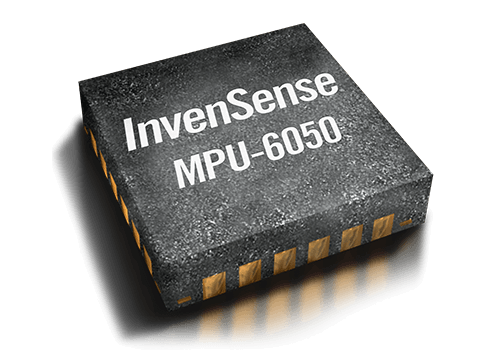
\includegraphics[height=3cm]{assets/mpu-6050.png}
    \caption{MPU-6050 \cite{mpu6050}.}
    \label{fig:mpu-6050}
\end{figure}

\subsubsection{Motor Driver}
The TB6612FNG dual motor driver (shown in Fig. \ref{fig:tb6612fng}) allows independent control of two DC motors. It uses a MOSFET H-bridge for bidirectional and Pulse Width Modulation (PWM) based motor speed control. Fig. \ref{fig:tb6612fng_plot} shows that each channel of the TB6612FNG can deliver up to 0.85A of current continuously. Furthermore, it consists of integrated over-current protection and thermal shutdown features for enhance reliability \cite{TB6612FNG}.

\begin{figure}[h]
	\centering
	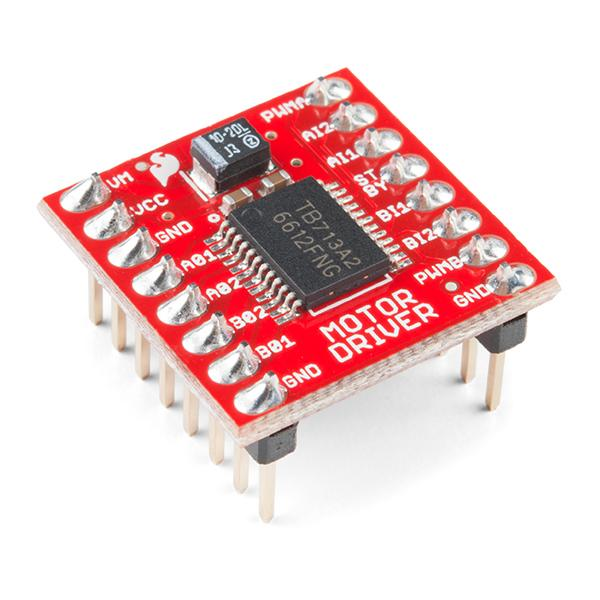
\includegraphics[height=3cm]{assets/TB6612FNG.jpg}
	\caption{TB6612FNG\cite{TB6612FNG_photo}.}
	\label{fig:tb6612fng}
\end{figure}

\begin{figure}[H]
	\centering
	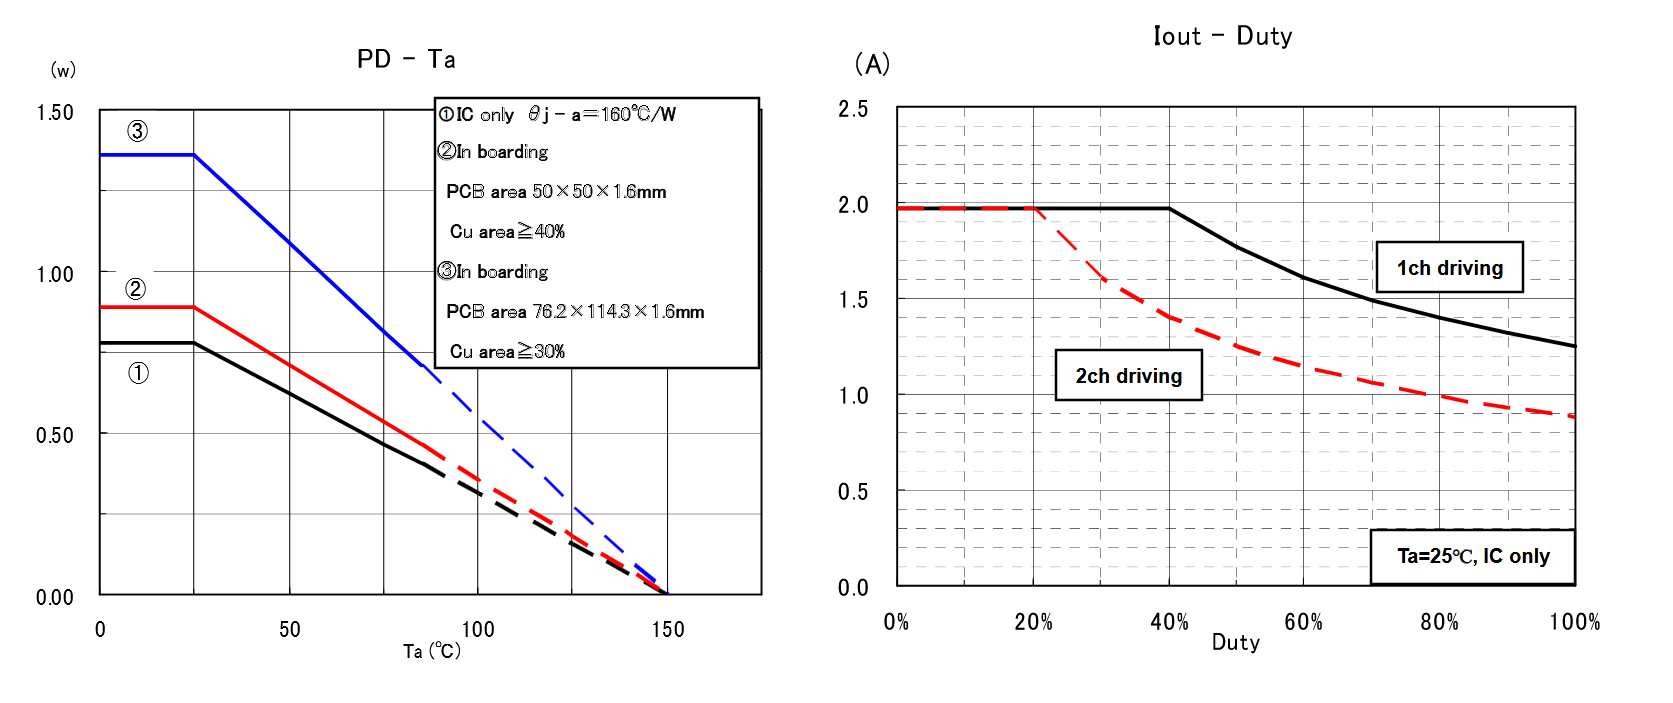
\includegraphics[height=6cm]{assets/TB6612FNG_target_characteristics}
	\caption{Target characteristics for TB6612FNG \cite{TB6612FNG}.}
	\label{fig:tb6612fng_plot}
\end{figure}

Instead of using two separate MCU pins for direction control, a single pin can be used with an inverted Schmitt trigger to generate the complementary signal automatically. For this purspose SN74LVC2G14 (shown in Fig. \ref{fig:SN74LVC2G14}) is used. It also enhances motor control by improving signal stability (similar to what is shown in Fig. \ref{fig:schmitt_trigger_hysteresis}).  
\begin{figure}[h]
	\centering
	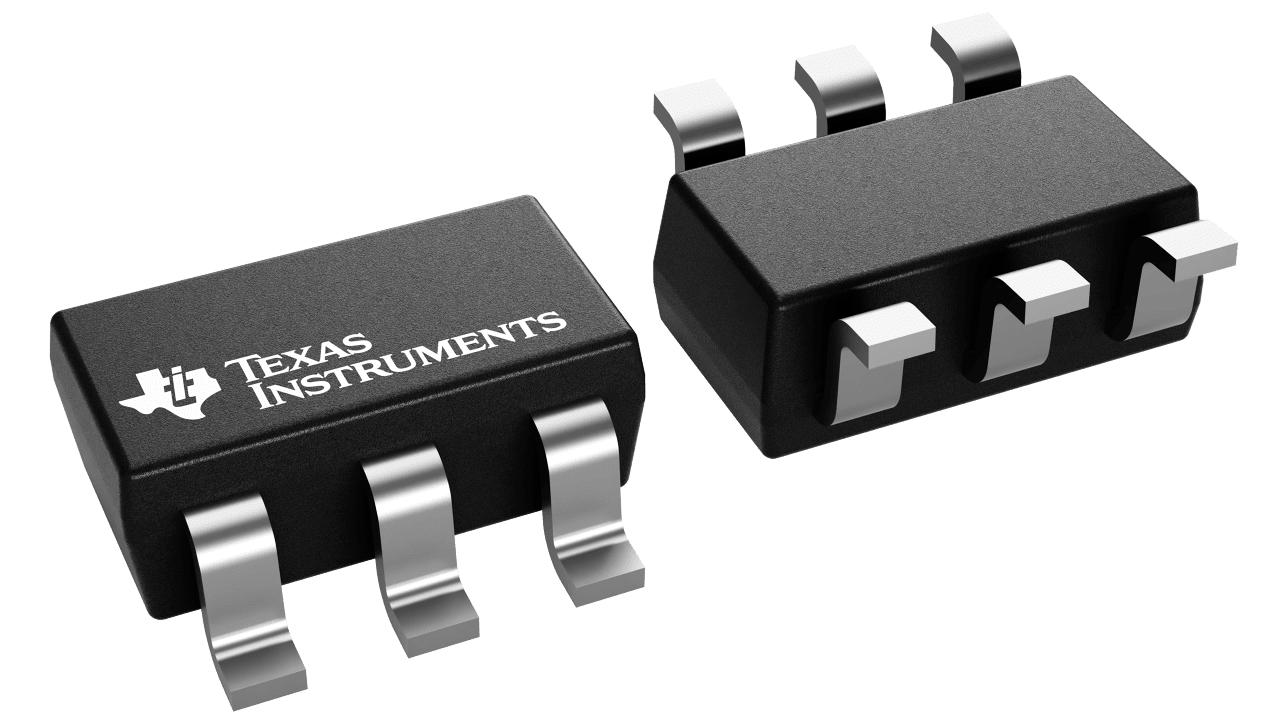
\includegraphics[height=2cm]{assets/SN74LVC2G14.png}
	\caption{SN74LVC2G14\cite{SN74LVC2G14}.}
	\label{fig:SN74LVC2G14}
\end{figure}

\begin{figure}[H]
	\centering
	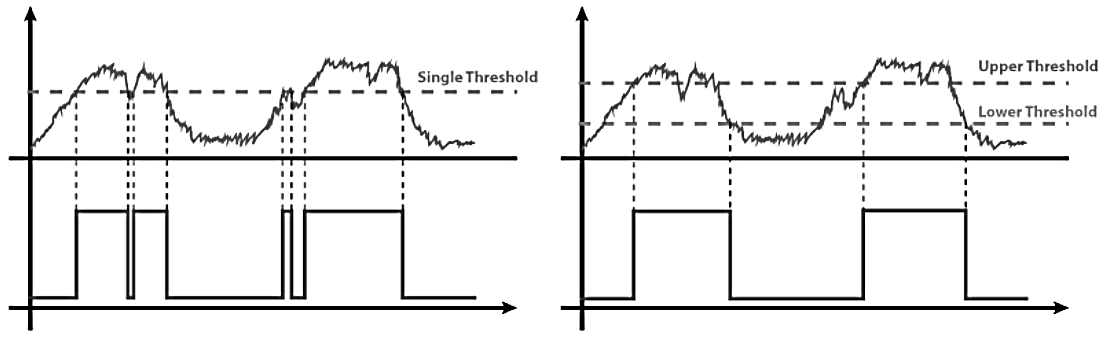
\includegraphics[height=4cm]{assets/schmitt_trigger_hysteresis.png}
	\caption{Schmitt trigger output without hysteresis (left) and with hysteresis (right) \cite{schmitt_trigger_hysteresis}.}
	\label{fig:schmitt_trigger_hysteresis}
\end{figure}

\subsubsection{Drive Motors}
The drive system employs NNHYTECH GA37 520 DC motors (37mm diameter, 12V, 360 RPM) equipped with Hall effect encoders (shown in Fig. \ref{fig:dc-motor}) \cite{dc-motor}. These motors feature a reduction gearbox, which enhances torque output while maintaining controlled rotational speed, making them well-suited for applications requiring precise motion control. The Hall effect encoders generate quadrature signals, enabling accurate measurement of speed and position. Motors from NHYTech were in this case.
\begin{figure}[H]
    \centering
    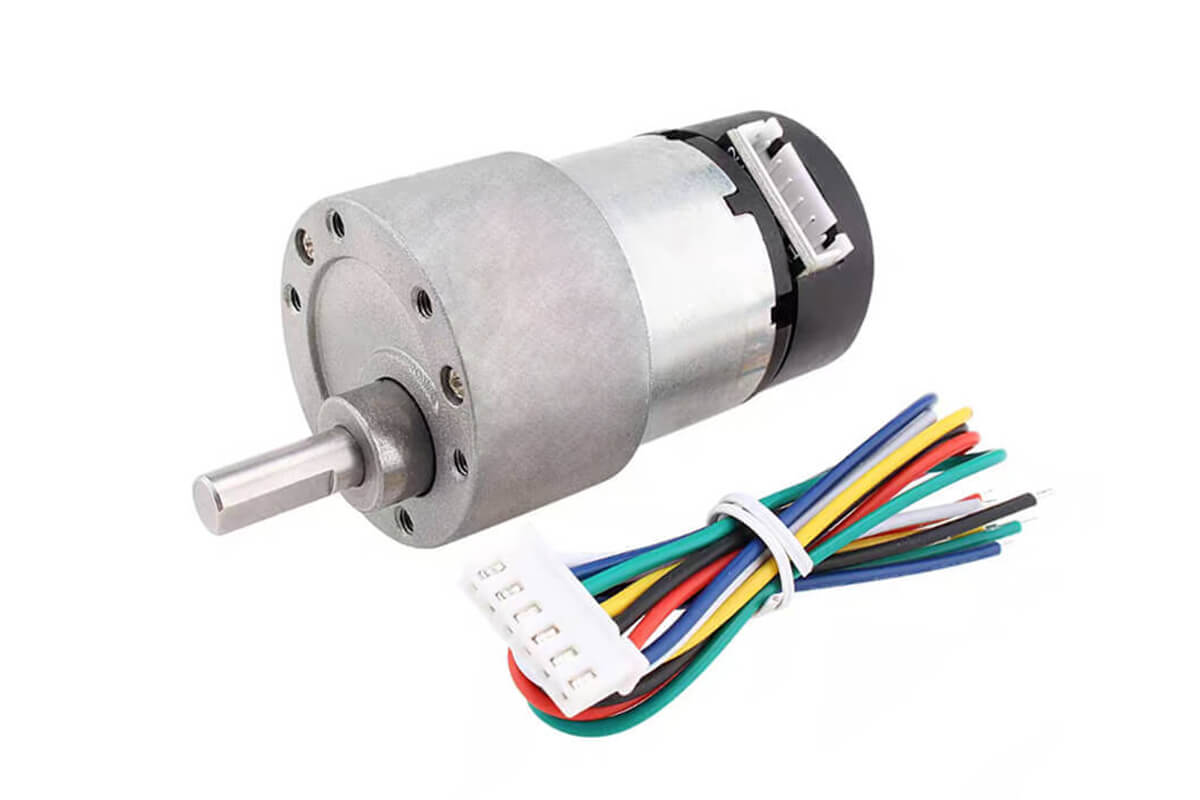
\includegraphics[height=4cm]{assets/dc-motor-with-encoder.jpg}
    \caption{Similar construction motors were used in this project \cite{dc-motor}.}
    \label{fig:dc-motor}
\end{figure}

\subsubsection{Ultrasonic Distance Sensor}
The HC-SR04 is an ultrasonic distance sensor used for measuring the distance to an obstacle by sending an ultrasonic pulse and measuring the time it takes for the echo to return. It operates based on the principle of time-of-flight of sound waves, with a known speed of sound in air.
\begin{figure}[H]
    \centering
    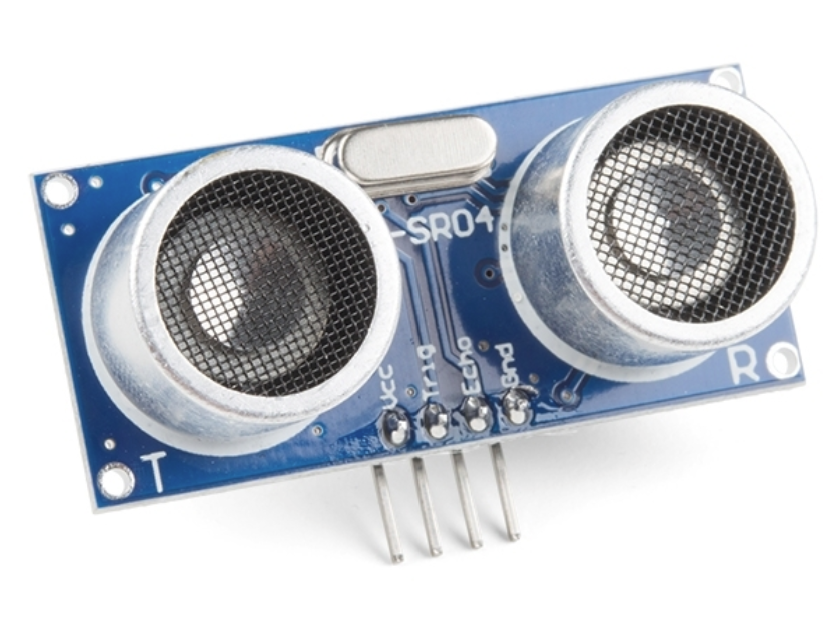
\includegraphics[width=0.25\linewidth]{assets/Ultrasonic-HC-SR04.png}
    \caption{Ultrasonic distance sensor by  Sparkfun electronics \cite{ultra-sonic}.}
    \label{fig:ultra-sonic}
\end{figure}

\subsubsection{Infrared Sensing}
The robot is equipped with infrared proximity sensors at the front-left and front-right directions using the Everlight Elec IR Receiver (IRM-56384) and the Infrared LED (IR204C-A). These sensors detect obstacles by transmitting a modulated infrared signal and detecting its reflection.
\begin{figure}[H]
\begin{subfigure}{0.5\textwidth}
    \centering
    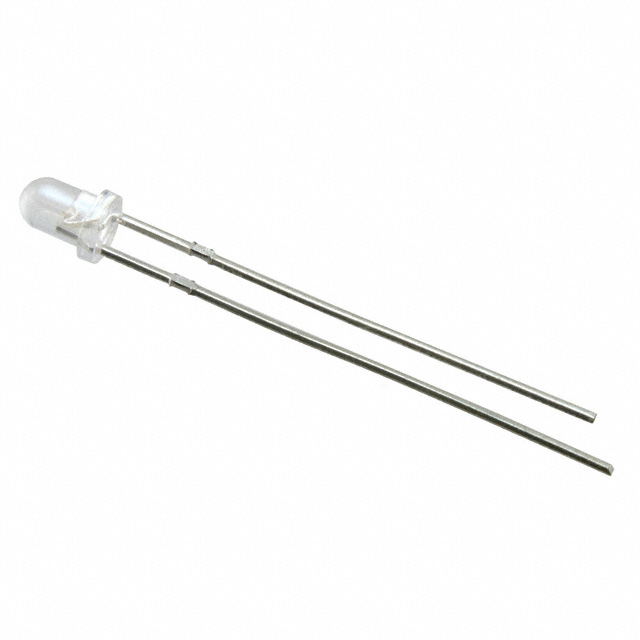
\includegraphics[height=3cm]{assets/HIR204C.jpg} 
    \caption{IR204C-A \cite{ir-led}.}
    \label{fig:ir-led}
\end{subfigure}
\begin{subfigure}{0.5\textwidth}
    \centering
    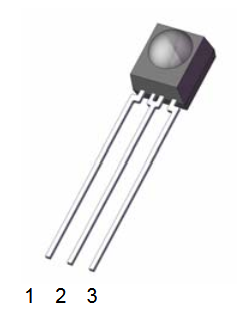
\includegraphics[height=3cm]{assets/ir-receiver.png} 
    \caption{IRM-56384 \cite{ir-receiver}.}
    \label{fig:ir-receiver}
\end{subfigure}
    \caption{LED-Emitter (a) and Infrared LED Reciever (b).} % Caption for the whole figure
    \label{fig:ir-sensors}
\end{figure}

\subsection{Bluetooth}
The BT16 4.2 Bluetooth transparent transmission module is a cutting-edge component that leverages the advanced capabilities of the Airoha ABI 602 single chip, which is compliant with the Bluetooth 4.2 BLE standard. This module facilitates GATT-based Bluetooth data transmission through its integrated data transparent transmission service, ensuring efficient and reliable communication. One of the key features of the BT16 module is its support for serial command mode, which enables seamless interaction between the external microcontroller unit (MCU) and the Bluetooth module. This functionality allows users to configure various parameters and exert control over the module via serial port commands. Users can modify essential settings such as the UUID, change the Bluetooth device name, and manage Bluetooth disconnection processes. 


\begin{figure}[H]
	\centering
	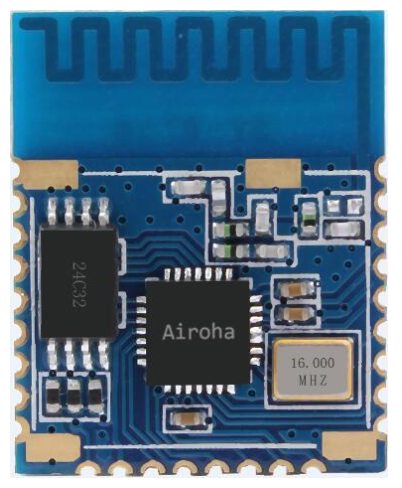
\includegraphics[height=3cm]{assets/BT16Module.png}
	\caption{Ultrasonic distance sensor by  Sparkfun electronics \cite{bluetooth}.}
	\label{fig:bluetooth}
\end{figure}


\subsubsection{Power Supply considerations}
This custom-designed battery box provides a portable and rechargeable power solution for the Elegoo robot \cite{battery}. Housing two 18650 LiPo batteries (likely connected in series), it delivers a regulated output to power the robot's various components. The integrated Battery Management System (BMS) ensures safe operation by providing overcharge, over-discharge, over-current, and short-circuit protection. A power switch allows for complete disconnection, while a USB charging port and status indicator LED simplify recharging and monitoring.  

\begin{figure}[H]
	\centering
	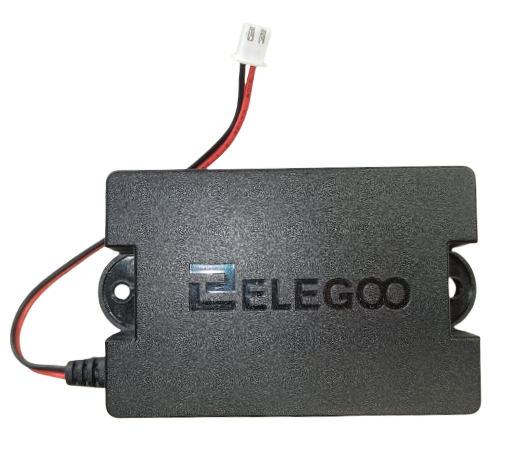
\includegraphics[height=6cm]{assets/Battery.png}
	\caption{ELEGOO battery pack with charger.}
	\label{fig:battery}
\end{figure}



\section{Mathematical Modelling}
$$
\begin{bmatrix}
    \dot{x} \\
    \ddot{x} \\
    \dot{\psi} \\
    \ddot{\psi}
\end{bmatrix}
= A
\begin{bmatrix}
    x \\
    \dot{x} \\
    \psi \\
    \dot{\psi}
\end{bmatrix}
+ B u_{input}
$$


\section{Software Implementation}
\subsection{Firmware Overview}
\begin{figure}[h]
	\centering
	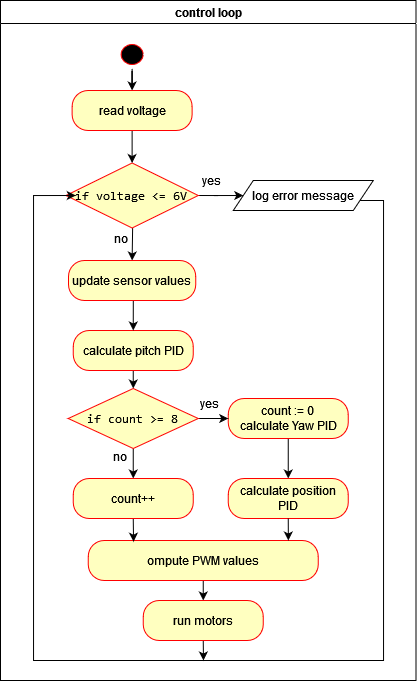
\includegraphics[width=0.5\linewidth]{assets/Control_Loop.png}
	\caption{A simplified block diagram of the control loop. }
	\label{fig:control-loop}
\end{figure}

\section{Sensor Fusion for Self-Balancing Robot using MPU6050}
\subsection{Introduction}
Self-balancing robots require accurate estimation of their tilt angle for effective control. The MPU6050, a widely used Inertial Measurement Unit (IMU), provides raw accelerometer and gyroscope data. However, due to individual sensor limitations, direct usage of these readings is unreliable. Sensor fusion techniques like the Complementary Filter and Kalman Filter help in obtaining a stable and accurate tilt angle

\subsubsection{Microcontroller}
The ATmega328P (shown in Fig. \ref{fig:ATmega328p}) is a popular microcontroller from Microchip Technology, widely used in embedded systems and electronics projects. With a 16 MHz clock speed, 32 KB of flash memory, 2 KB of SRAM, and 1 KB of EEPROM \cite{atmega_microchip}, the ATmega328P provides ample resources for this projects application. 

The ATMEGA328P is also used in the Arduino Nano (shown in Fig. \ref{fig:arduino_nano}), a widely adopted development board known for its low cost and open-source ecosystem \cite{arduino_nano}. The combination of affordability and extensive community support makes it an ideal choice for rapid prototyping and academic research, ensuring easy integration with various sensors and motor drivers. 

\begin{figure}[H]
	\centering
	\subfloat[ATMEGA328P \cite{atmega_microchip}.]{
		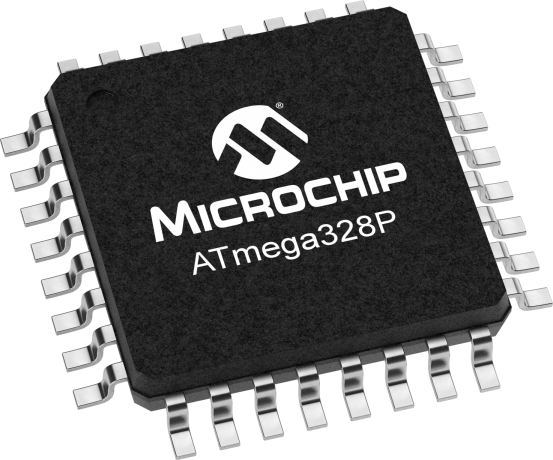
\includegraphics[height=3cm]{assets/ATmega328p.png}
		\label{fig:ATmega328p}
	}
	\qquad
	\subfloat[Arduino Nano \cite{arduino_nano}.]{
	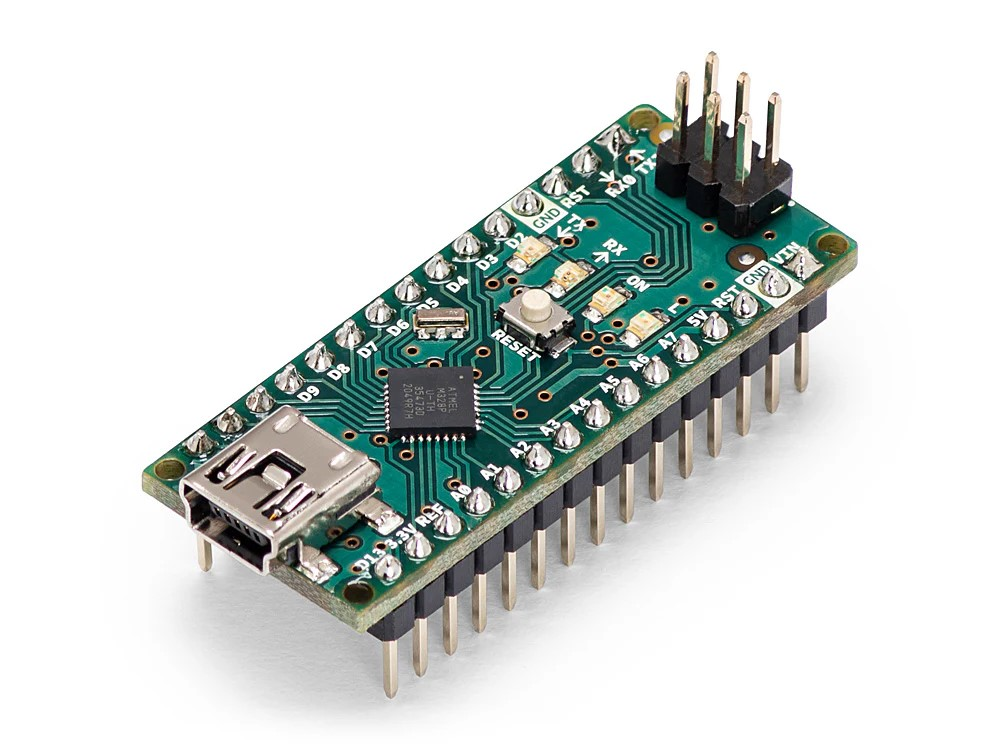
\includegraphics[height=3cm]{assets/arduino_nano.jpg}
	\label{fig:arduino_nano}
	} 
	\label{fig:ATmega328p_and_arduino_nano}
	\caption{}
\end{figure}

\subsubsection{Inertial Measuring Unit}
The MPU6050 is a widely used six-axis sensor that integrates a three-axis gyroscope and a three-axis accelerometer on a single chip, making it essential for motion tracking and stabilization applications (shown in Fig. \ref{fig:mpu-6050}). Its compact design and built-in Digital Motion Processor (DMP) enable real-time processing of sensor data, which is crucial for robotics, drones, and wearable devices.
In applications like self-balancing robots, it provides accurate orientation and acceleration data necessary for maintaining stability. 

\begin{figure}[H]
	\centering
	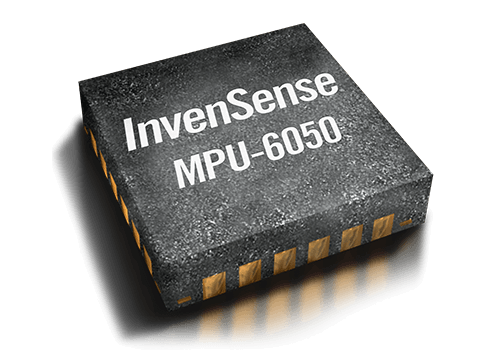
\includegraphics[height=3cm]{assets/mpu-6050.png}
	\caption{MPU-6050 \cite{mpu6050}.}
	\label{fig:mpu-6050}
\end{figure}


\subsection{Working of MPU6050}
The MPU6050 is a 6-axis IMU that provides:
\begin{itemize}
	\item Accelerometer Data: Measures acceleration in X, Y, and Z axes. It helps in estimating tilt based on gravitational force.
	\item Gyroscope Data: Measures angular velocity around X, Y, and Z axes. Integration of gyroscope readings over time provides the tilt angle.
\end{itemize}

\subsubsection{Reading Raw Sensor Data}
The \texttt{read\_mpu\_6050\_data()} function reads raw data from the MPU6050 sensor:
\begin{itemize}
	\item It requests 14 bytes of data from the sensor, covering the accelerometer, gyroscope, and temperature sensor readings.
	\item The data is stored in respective variables after combining the high and low bytes. 
	\item If data retrieval fails, an error message is displayed.
\end{itemize}
\begin{lstlisting}[style=cppstyle2]
void mpu6050Base::read_mpu_6050_data() {
	Wire.beginTransmission(mpu6050_addr);
	Wire.write(0x3B);
	Wire.endTransmission();
	Wire.requestFrom(mpu6050_addr, (uint8_t)14);
	
	if (Wire.available() >= 14) {
		acc_x = Wire.read() << 8 | Wire.read();
		acc_y = Wire.read() << 8 | Wire.read();
		acc_z = Wire.read() << 8 | Wire.read();
		temperature = Wire.read() << 8 | Wire.read();
		gyro_x = Wire.read() << 8 | Wire.read();
		gyro_y = Wire.read() << 8 | Wire.read();
		gyro_z = Wire.read() << 8 | Wire.read();
	} else {
		ERROR_PRINT("Data cannot be read from MPU6050!");
	}
	
}
\end{lstlisting}

\subsubsection{Issues with Raw Sensor Data}
\begin{itemize}
\item \textbf{Accelerometer Noise}: While providing an absolute angle reference, accelerometer readings are noisy and susceptible to external forces.
\item \textbf{Gyroscope Drift}: Over time, integration errors cause drift, leading to inaccurate angle estimation.
To overcome these issues, sensor fusion techniques are applied.
\end{itemize}


\subsection{Complementary Filter}
The complementary filter is a simple yet effective method for sensor fusion \cite{rabbany_design_2021} \cite{10193276} \cite{1174486}. It blends high-frequency data from the gyroscope with low-frequency data from the accelerometer:

\subsubsection{Mathematical Model}
Raw accelerometer readings $A_y$ and $Az$ can be used to calculate tilt angle using following equation:
\begin{equation}
\theta_{acc} = \text{arctan} \left(A_y/Az  \right) \label{eq:eq}
\end{equation}
Similarly, using raw angular velocity data from the gyroscope $\omega_{x}$,
\begin{equation}
	\begin{aligned}
		\dot{\theta}_{gyro}(t) &= - \omega_{x,bias}(t) \\ \label{eq:state_eq_1}
		\dot{\omega}_{x,bias}(t) &= 0
	\end{aligned}
\end{equation}
In these equations, $\theta(t)$ represents the measured angle of the system, and $\omega_{\text{gyro,bias}}(t)$ represents the bias of the gyroscope. The first equation models how the angle evolves over time, influenced by the constant gyroscope bias. The second equation indicates that the gyroscope bias remains constant over time. The sampling time interval $\Delta t$ and previous angle value $\theta_{previous}$ can be used to calculate tilt angle using following equation:
\begin{equation}
\theta_{gyro} = \theta_{previous, gyro} + \omega_{gyro} \Delta t \label{eq:eq}
\end{equation}
Then the final estimated angle $\theta_{estimate}$ is calculated as:
\begin{equation}
	\theta_{estimate} = \alpha \ \theta_{gyro} + (1 - \alpha) \ \theta_{acc} \label{eq:eq}
\end{equation}
Where $\alpha$ is the filter coefficient, $\omega$ is the angular velocity from the gyroscope, and $\theta_{acc}$ is the angle from the accelerometer.

\subsubsection{Initial Calibration}
The \texttt{init()} function is responsible for initializing the MPU6050 sensor and performing gyroscope calibration:
\begin{itemize}
	\item The I2C communication is established with the sensor, and an acknowledgment is checked to ensure proper connection.
	\item The function sets up the MPU6050 registers using \texttt{setup\_mpu\_6050\_registers()}, configuring the power management and sensitivity ranges for both the accelerometer and gyroscope.
	\item Gyroscope calibration is performed by collecting multiple readings and averaging them to calculate offsets for the X, Y, and Z axes. These offsets help reduce sensor drift.
\end{itemize}

\begin{lstlisting}[style=cppstyle2]
void mpu6050Base::init() {
	Wire.beginTransmission(mpu6050_addr);
	if (Wire.endTransmission() != 0) {
		ERROR_PRINT("MPU6050 not connected!");
		return;
	}
	setup_mpu_6050_registers();
	
	for (int i = 0; i < CALIBRATION_SAMPLES; i++) {
		read_mpu_6050_data();
		gyro_x_cal += gyro_x;
		gyro_y_cal += gyro_y;
		gyro_z_cal += gyro_z;
		delay(3);
	}
	gyro_x_cal /= CALIBRATION_SAMPLES;
	gyro_y_cal /= CALIBRATION_SAMPLES;
	gyro_z_cal /= CALIBRATION_SAMPLES;
}
\end{lstlisting}

\subsubsection{Calculating Angles}
The \texttt{calculate()} function processes raw sensor data to determine pitch and roll angles:
\begin{itemize}
	\item Gyroscope readings are corrected using calibration offsets to remove bias.
	\item Angular velocity is integrated over time to estimate orientation changes.
	\item The accelerometer-derived angles are computed from the total acceleration vector using trigonometric transformations.
	\item A complementary filter is applied to blend gyroscope and accelerometer readings, mitigating drift and noise while enhancing stability.
\end{itemize}

\begin{lstlisting}[style=cppstyle2]
void mpu6050Base::calculate() {
	read_mpu_6050_data();
	
	gyro_x -= gyro_x_cal;
	gyro_y -= gyro_y_cal;
	gyro_z -= gyro_z_cal;
	
	angle_pitch += gyro_x * 0.0000611;
	angle_roll += gyro_y * 0.0000611;
	
	angle_pitch += angle_roll * sin(gyro_z * 0.000001066);
	angle_roll -= angle_pitch * sin(gyro_z * 0.000001066);
	
	acc_total_vector = sqrt((acc_x * acc_x) + (acc_y * acc_y) + (acc_z * acc_z));
	
	angle_pitch_acc = asin((float)acc_y / acc_total_vector) * 57.296;
	angle_roll_acc = asin((float)acc_x / acc_total_vector) * -57.296;
	
	if (set_gyro_angles) {
		angle_pitch = angle_pitch * 0.9996 + angle_pitch_acc * 0.0004;
		angle_roll = angle_roll * 0.9996 + angle_roll_acc * 0.0004;
	} else {
		angle_pitch = angle_pitch_acc;
		angle_roll = angle_roll_acc;
		set_gyro_angles = true;
	}
	
	angle_pitch_output = angle_pitch_output * 0.9 + angle_pitch * 0.1;
	angle_roll_output = angle_roll_output * 0.9 + angle_roll * 0.1;
	
}
\end{lstlisting}


\subsubsection{Results}

\begin{figure}[H]
	\centering
	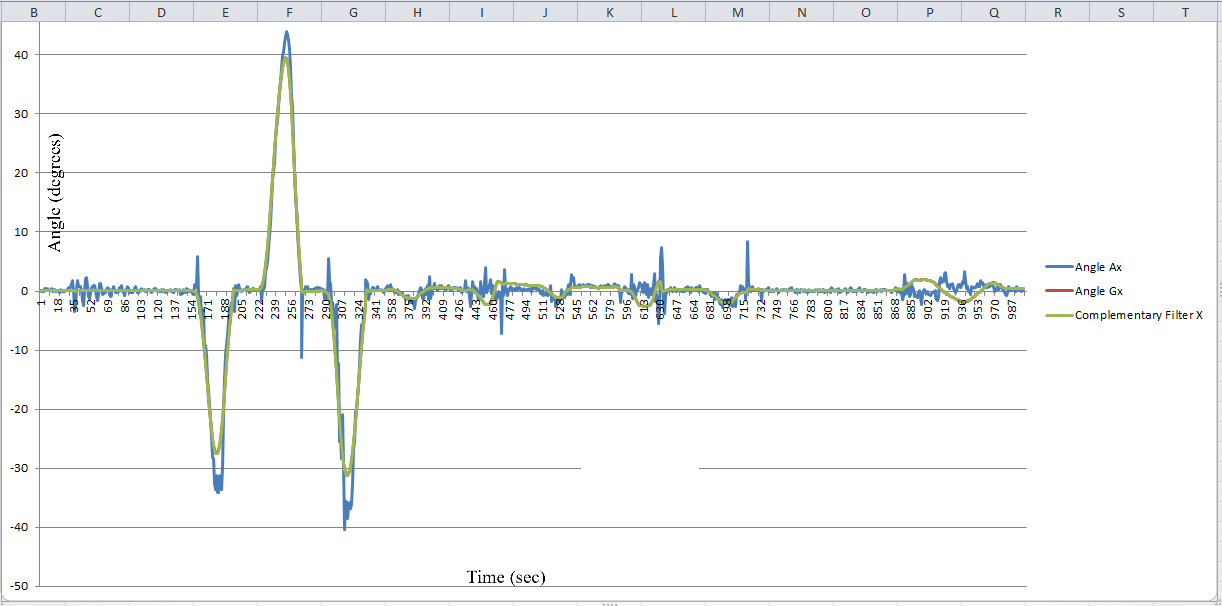
\includegraphics[height=8cm]{assets/compl_filter_0.9.png}
	\caption{Pitch angle caluclated using a complementary filter with $\omega = 0.9$.}
	\label{fig:battery}
\end{figure}


\subsection{Extended Kalman Filter (EKF)}
The Kalman filter (KF) provides a more sophisticated approach, estimating the true state of the system by minimizing the mean of the squared error. It involves prediction and update steps. However,  assumes that both the process and measurement models are linear. However, many real-world systems, such as robotic motion and sensor fusion, exhibit inherent nonlinearities. When linearization is not feasible, the standard KF becomes inaccurate. 

To address this limitation, the Extended Kalman Filter (EKF) extends the KF to nonlinear systems by employing a first-order Taylor series expansion. This method approximates the nonlinear system dynamics and measurement models with locally linearized representations, allowing the filter to be applied in scenarios where exact linearization is not feasible.

The EKF is an extension of the Kalman Filter for nonlinear systems, utilizing first-order Taylor series expansion to linearize process and measurement models. EKF maintains a Gaussian belief over the state, updating it through a prediction-correction cycle. The Jacobian matrices of the system dynamics and measurement functions are used to approximate state transitions and measurement updates. Its advantages include handling nonlinearities, fusing multi-sensor data, and improving estimation accuracy in noisy environments. 

\subsubsection{General State Equation}
For non-linear system, with Stochastic disturbances:
\begin{equation}
\begin{aligned}
	\dot{\underline{x}}(t) &= f\left( \underline{x}(t), \underline{u}(t) \right) + \underline{d}(t) \\
	\underline{y}(t) &= h\left( \underline{x}(t) \right) + \underline{n}(t)
\end{aligned}
\end{equation}
where,
\begin{itemize}
	\item $ \dot{\underline{x}}(t) $: This represents the time derivative of the state vector $ \underline{x}(t) $, indicating how the state evolves over time.
	\item $ f $: This is a nonlinear function that describes the system dynamics, taking the current state $ \underline{x}(t) $ and the control input $ \underline{u}(t) $ as arguments. It captures how the state changes based on the current state and control inputs.
	\item $ \underline{d}(t) $: This term represents stochastic disturbances (or process noise) affecting the state dynamics, typically modeled as a zero-mean Gaussian noise.
	\item $ y(t) $: This is the measurement vector at time $ t $, representing the observed outputs of the system. It is the data collected from sensors or measurement devices.
	\item $ h $: This is a nonlinear measurement function that maps the true state vector $ \underline{x}(t) $ to the measurement space. It describes how the state influences the measurements. The function $ h $ can be complex and may involve various transformations of the state variables.
	\item $ n(t) $: This term represents measurement noise, which is also typically modeled as zero-mean Gaussian noise. It accounts for inaccuracies in the measurements due to sensor errors, environmental conditions, or other random factors that can affect the observed data.
\end{itemize}

\subsubsection{State Estimation}
For a non-linear system the state form is as follows,
\begin{equation}
\begin{aligned}
	\dot{\hat{\underline{x}}}(t) &= f\left( \underline{\hat{x}}(t), \underline{u}(t) \right) + \underline{K}\left( y(t) - \hat{y}(t) \right) \\
	\hat{y}(t) &= h\left( \underline{\hat{x}}(t) \right)  \label{eq:eq}
\end{aligned}
\end{equation}
The Kalman gain $\underline{K}$ is computed to optimally balance estimation uncertainty and measurement noise. To achieve this, the system is first linearized around the current state estimate by computing the Jacobians of the process and measurement models. To linearize the system around the current state estimate, the Jacobian matrices, which represent the first-order partial derivatives of the nonlinear functions, are computed as follows:
\begin{equation}
\underline{A}(t) = \frac{\mathrm{d}f}{\mathrm{d}\underline{x}} \bigg|_{\underline{\hat{x}}(t), \underline{u}(t)} \quad \text{and} \quad
\underline{C}(t) = \frac{\mathrm{d}h}{\mathrm{d}\underline{x}} \bigg|_{\underline{\hat{x}}(t)}  \label{eq:eq}
\end{equation}
where $\underline{A}(t)$ represents the partial derivatives of the state dynamics function $f$ and $\underline{C}(t)$ represents the partial derivatives of the measurement function $h$.
\begin{figure}[h]
	\centering
	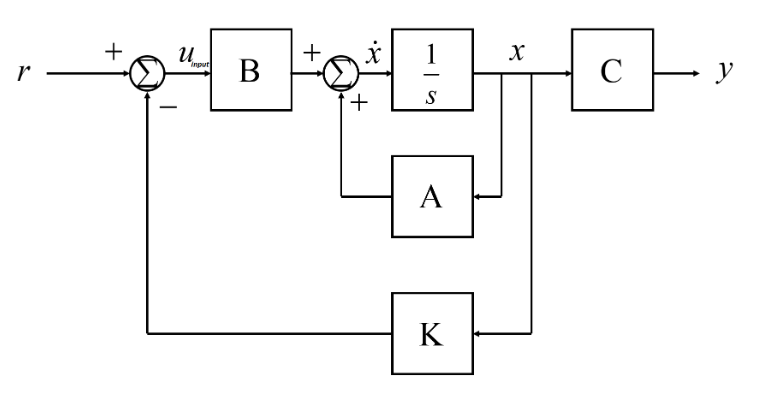
\includegraphics[height=5cm]{assets/block_representation_kalman_filter.png}
	\caption{Block representation of state space system showing the system matrices $A$, $B$ and $C$ as well as the gain matrix $K$.}
	\label{fig:block_representation_kalman_filter}
\end{figure}
\subsubsection{Covraince Matrix}
The evolution of the state estimation covariance matrix follows the continuous-time Riccati equation, given by:
\begin{equation}
\dot{P}(t) = \underline{A}(t) P(t) + P(t) \underline{A}^T(t) + Q - P(t) \underline{C}^T(t) R^{-1} \underline{C}(t) P(t)  \label{eq:eq}
\end{equation}
Where, 
\begin{itemize}
	\item $\dot{P}(t)$: his represents the time derivative of the covariance matrix $\dot{P}(t)$, which quantifies the uncertainty in the state estimate over time.
	\item $\underline{A}(t)$: This is the state transition matrix, which describes how the state evolves from one time step to the next.
	\item $Q$: This is the process noise covariance matrix, representing the uncertainty in the process model.
	\item $\underline{C}(t)$: This is the measurement matrix, which relates the state to the measurements.
	\item $R$: This is the measurement noise covariance matrix, representing the uncertainty in the measurements.
\end{itemize}
The Kalman filter is initialized with an initial covariance matrix:
\begin{equation}
	P(0) = \mathbf{E}(\Delta\underline{x}(0) \Delta\underline{x}^T(0))  \label{eq:eq}
\end{equation}
The optimal Kalman gain, balancing estimation uncertainty and measurement noise, is given by:

\begin{equation} \underline{K}(t) = P(t) \underline{C}^T R^{-1} \end{equation}
The time-discrete Kalman filter state update equations are:
\begin{equation}
	\begin{aligned}
		\underline{x}_{k} &= \underline{A} \underline{x}_{k-1} + \underline{B} \underline{u}_{k} + \underline{d}_{k-1} \\
		\underline{y}_{k} &= \underline{C} \underline{x}_{k} + \underline{n}_{k}  \label{eq:eq}
	\end{aligned}
\end{equation}
where $\underline{x}_k$ is the state vector, $\underline{B}$ the control input matrix, and $\underline{y}_k$ the measurement vector. The discrete state-space representation is:
\begin{equation}
	\begin{aligned}
		\underline{\dot{x}}(t) = \underline{A}.\underline{x}(t) + \underline{B}.\underline{u}(t) \\
		\underline{y}(t) = \underline{C}.\underline{x}(t) + \underline{D}.\underline{u}(t)  \label{eq:eq}
	\end{aligned}
\end{equation}
The state covariance matrix is:
\begin{equation}
	\mathbf{P}_k = \begin{bmatrix} P_{00} & P_{01} \\ P_{10} & P_{11} \end{bmatrix}  \label{eq:eq}
\end{equation}
where $P_{00}$ represents uncertainty in the angle estimate and $P_{11}$ in gyroscope bias. The Kalman gain is computed as:
\begin{equation}
	\begin{aligned}
		\underline{K}_{k} &= \underline{P}_{k}^- \ \underline{C}^T ( \underline{C} \ \underline{P}_{k}^-\ \underline{C}^T  +\underline{R})^{-1} \\ \\
		\mathbf{K}_k &= \begin{bmatrix} \frac{ P_{00} }{ P_{00}  
				+ R_{angle}} \\ \frac{ P_{10} }{ P_{00}  
				+ R_{angle}} \end{bmatrix}
	\end{aligned}  \label{eq:eq}
\end{equation}
Following the prediction step, the measurement update step refines the state estimate using the Kalman gain, which is derived to minimize the posterior estimation error covariance (see Appendix \ref{appendix:B} for detailed calculations):
\begin{equation}
	\begin{aligned}
		\underline{P}_{k} &= \ (\underline{I} - \underline{K}_{k} \ \underline{C}) \ \underline{P}_{k}^- \label{eq:eq}
	\end{aligned}
\end{equation}


\subsection{Software Implementation of EKF}
For the implementation of the Extended Kalman Filter (EKF), we utilized the Kalman filter library developed by Kristian Lauszus~\cite{github_kalman_filter}. This library was modified in accordance with the GNU General Public License to meet the specific requirements of our project.
\begin{lstlisting}[style=cppstyle2]
#include <Arduino.h>

class KalmanFilter {
 private:
  float m_dt, m_Q_angle, m_Q_gyro, m_R_angle, m_C_0;
  float q_bias = 0, angle_err = 0;
  float P[2][2] = {{1, 0}, {0, 1}}; // Covariance matrix
  float K_0 = 0, K_1 = 0;

 public:
  float angle = 0;

KalmanFilter(float dt, float Q_angle, float Q_gyro, float R_angle, float C_0)
: m_dt(dt), m_Q_angle(Q_angle), m_Q_gyro(Q_gyro), m_R_angle(R_angle), m_C_0(C_0) {}

float getAngle(float measured_angle, float measured_gyro) {
	// Predict
	angle += (measured_gyro - q_bias) * m_dt;
	angle_err = measured_angle - angle;
	
	// Update covariance matrix
	P[0][0] += m_Q_angle - P[0][1] - P[1][0];
	P[0][1] -= P[1][1];
	P[1][0] -= P[1][1];
	P[1][1] += m_Q_gyro;
	
	// Compute Kalman gain
	float E = m_R_angle + m_C_0 * P[0][0];
	K_0 = (m_C_0 * P[0][0]) / E;
	K_1 = (m_C_0 * P[1][0]) / E;
	
	// Update state
	angle += K_0 * angle_err;
	q_bias += K_1 * angle_err;
	
	// Update covariance matrix
	float C0_P00 = m_C_0 * P[0][0];
	P[0][0] -= K_0 * C0_P00;
	P[0][1] -= K_0 * P[0][1];
	P[1][0] -= K_1 * P[0][0];
	P[1][1] -= K_1 * P[0][1];
	
		return angle;
	}
};
\end{lstlisting}

\section{Cascaded PID Control Loop}

The algorithm utilizes cascade Proportional–Integral–Derivative (PID) control loop to maintain balance and control the robot's movement in real time. The balancing is achieved by continuously monitoring and adjusting its state using sensor feedback. The key sensor inputs include the robot's pitch angle, gyro data and motor's encoder values, which provide information on the robot's orientation, angular velocities and position.The algorithm utilizes cascade PID control loops to maintain balance and control the robot's movement in real time. The approach includes computing control outputs for pitch, yaw, and position periodically, which are then used to adjust the motor speeds by sending corresponding pulse-width-modulation (PWM) signals to the motor driver (see Fig. \ref{fig:control-loop}).

\begin{figure}[h]
	\centering
	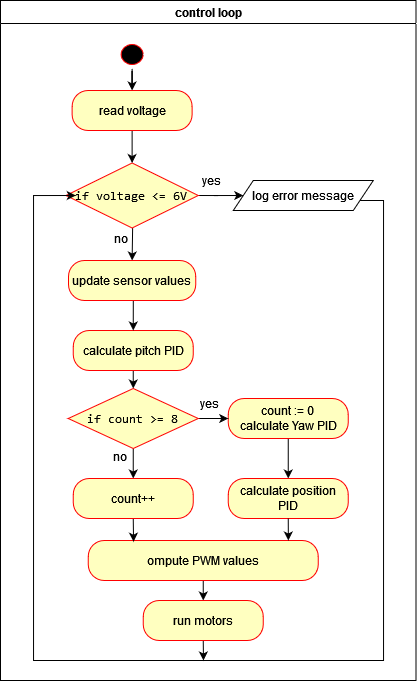
\includegraphics[width=0.5\linewidth]{assets/Control_Loop.png}
	\caption{A simplified block diagram of the control loop. }
	\label{fig:control-loop}
\end{figure}

As the pitch angle is more important for system stability, therefore it is updated more frequently (e.g. updated every cycle), while the PID output values for the yaw angle and position control are updated longer duration of time (e.g. after every 8th cycle).

\subsection{Basic PID Structure}
The PID controller output can be expressed mathematically as:

\begin{equation}
	u(t) = K_p e(t) + K_i \int_0^t e(\tau)d\tau + K_d \frac{d}{dt}e(t)
\end{equation}

Where:
\begin{itemize}
	\item $u(t)$ is the control signal
	\item $e(t)$ is the error signal
	\item $K_p$ is the proportional gain
	\item $K_i$ is the integral gain
	\item $K_d$ is the derivative gain
\end{itemize}



\subsection{Position Control Loop}
The outer loop manages the robot's position:

\begin{equation}
	\theta_{desired} = K_{px}(x_{desired} - x_{measured}) + K_{dx}\frac{d}{dt}(x_{desired} - x_{measured})
\end{equation}


\section{Implementation Considerations}
\subsection{Discrete Time Implementation}
For digital implementation, the PID controller is discretized:

\begin{equation}
	u[n] = K_p e[n] + K_i T_s \sum_{k=0}^n e[k] + K_d \frac{e[n] - e[n-1]}{T_s}
\end{equation}

Where $T_s$ is the sampling period.


\section{Tuning Methodology}
For tuning a general combination of Ziegler-Nichols method and practical tuning guidelines were used.
\subsection{Ziegler-Nichols Method}
The Ziegler-Nichols tuning method follows these steps:
\begin{enumerate}
	\item Set $K_i$ and $K_d$ to zero
	\item Increase $K_p$ until system oscillates with period $T_u$
	\item Record the ultimate gain $K_u$
	\item Calculate parameters:
	\begin{align*}
		K_p &= 0.6K_u \\
		T_i &= 0.5T_u \\
		T_d &= 0.125T_u
	\end{align*}
\end{enumerate}

\subsection{Practical Tuning Guidelines}
The general tuning guidelines are as follows:

\begin{itemize}
	\item Begin with small $K_p$ (= 10)
	\item Add derivative term ($K_d = 0.1K_p$)
	\item Fine-tune until stable
\end{itemize}


\subsection{Pitch PID Control:}
The pitch control loop ensures the robot maintains its upright position. The primary objective of the pitch controller is to minimize the deviation of the robot's pitch angle from a set-point, which is ideally zero degrees (i.e., upright). The pitch control output is calculated using the PD algorithm, where the error is the difference between the current pitch angle and the desired pitch angle. 
\begin{equation}
	\tau_{\theta,pid} = K_{p\theta}({\theta_{desired} - \theta_{measured}}) + K_{d\theta}\frac{d}{dt}(\theta_{desired} - \theta_{measured})
\end{equation}

Below is its code implementation:
\begin{lstlisting}[style=cppstyle]
inline void runPitchControl() {
	// Compute balance control output
	pitch_pid_output = kp_balance * (kalman.angle - 0) 
	+ kd_balance * (gyro_x  - 0);
}
\end{lstlisting}

\begin{itemize}
	\item \textbf{Proportional (P):} The proportional term is based on the current error (the pitch angle deviation from the desired value). A higher proportional gain causes the robot to respond more aggressively to larger deviations.
	\item \textbf{Derivative (D):} The derivative term anticipates future errors by considering the rate of change of the error (pitch angular velocity deviation from desired value). It provides a damping effect, which helps to reduce overshooting and oscillations.
	\item \textbf{Integral (I):} Because the system is inherently unstable when at desired upright position (steady state error can never be zero) thus adding the integral term is unnecessary. 
	
\end{itemize}

The output of the pitch PD controller ($\text{pitch\_pid\_output}$) is then used to adjust the robot's motor speeds to counteract any tilting or imbalance.

\subsection{Yaw Control:}
Yaw control is responsible for controlling the robot's rotational movement around its vertical axis. The yaw PID controller computes the control output based on the robot's angular velocity, which is measured by the gyroscope along the z-axis. The yaw control adjusts the motor speeds to achieve the desired rotational velocity, ensuring the robot maintains a stable heading.
\begin{equation}
	\tau_{\phi,pid} = K_{d\phi}\frac{d}{dt}(\phi_{desired} - \phi_{measured})
\end{equation}


Below is its code implementation:
\begin{lstlisting}[style=cppstyle]
inline void runYawControl(){
	yaw_pid_output = kd_turn * gyro_z;
}
\end{lstlisting}

Similar to pitch control, the yaw controller follows the PID principles:
\begin{itemize}
	\item \textbf{Proportional (P):} In order to calculate yaw angle, a high computational overhead is required, while yaw angle is not critical for balancing thus the proportional term is ignored.
	\item \textbf{Integral (I):} As the yaw angle is not calculated, therefore the integral term cannot be calculated as well.
	\item \textbf{Derivative (D):} The derivative term mitigates any excessive rate of change in yaw, preventing oscillations in the robot's rotation.
\end{itemize}

The yaw PID output ($\text{yaw\_pid\_output}$) is then combined with the pitch and position control outputs to compute the final motor PWM values.

\subsection{Position Control:}
Position control is implemented to ensure the robot moves smoothly and accurately along a path or to a target location. The encoder feedback from the left and right wheels is used to calculate the robot's displacement and speed. The position PID controller adjusts the motor speeds to minimize the error in position and velocity.
\begin{equation}
	\tau_{x,pid} = K_{px}(x_{desired} - x_{measured}) + K_{dx}\frac{d}{dt}(x_{desired} - x_{measured})
\end{equation}

Below is its code implementation:
\begin{lstlisting}[style=cppstyle]
inline void runPositionControl(){
	double encoder_speed = (left_encoder_position + right_encoder_position) * 0.5
	robot_position += encoder_speed;
	robot_position = constrain(robot_position, -3000, 3000);
	position_pid_output = - ki_position * robot_position - kd_position * encoder_speed;
}
\end{lstlisting}

To prevent integral windup:
\begin{equation}
	u_{limited} = \begin{cases}
		3000 & \text{if } u > 3000 \\
		u & \text{if } -3000 \leq u \leq 3000 \\
		-3000 & \text{if } u < -3000
	\end{cases}
\end{equation}

\begin{itemize}
	\item \textbf{Proportional (P):} The proportional term helps correct any immediate error in position by adjusting the motor speeds in response to the current position error.
	\item \textbf{Integral (I):} The integral term addresses any accumulated error in position that may arise due to external factors like friction or uneven terrain.
	\item \textbf{Derivative (D):} Because the position control does not require fast settling time, thus derivative term can be ignored in favour of faster calculation time.
	
\end{itemize}

The position control output ($\text{position\_pid\_output}$) is also factored into the final PWM values for motor control.

\subsection{Combining Control Outputs}

The final motor control is achieved by combining the outputs from all three PID controllers. The outputs from the pitch, yaw, and position PID controllers are used to calculate the motor speeds, which determine the robot's motion. Specifically, the following equation is used to compute the PWM values for the left and right motors:

\begin{align}
	\tau_{left,motor} &= \tau_{\theta,pid} - \tau_{\phi,pid} - \tau_{x,pid} \\
	\tau_{right,motor} &= \tau_{\theta,pid} + \tau_{\phi,pid} - \tau_{x,pid}
\end{align}

Below is its code implementation:
\begin{lstlisting}[style=cppstyle]
pwm_left = pitch_pid_output - yaw_pid_output - position_pid_output;
pwm_right = pitch_pid_output + yaw_pid_output - position_pid_output;
\end{lstlisting}

These calculated PWM values are then sent to the motor drivers to adjust the robot's movement and balance.

\subsection{Conclusion}

The use of PID controllers for pitch, yaw, and position control enables the robot to maintain balance and navigate effectively. The proportional, integral, and derivative terms in each PID loop allow the system to respond to real-time errors, minimize steady-state deviations, and anticipate future errors, leading to smooth and precise control of the robot's motion. The integration of these PID controllers is fundamental to the robot's stability and performance.



\subsection{Front Obstacle Detection}
The Ultrasonic distance measuring sensor is used to detect the obstacle in front of the robot.

\subsection{Ultrasonic Working Principle}
The sensor consists of a \textbf{transmitter} and a \textbf{receiver}:
\begin{itemize}
	\item The transmitter emits an ultrasonic pulse (40 kHz).
	\item The pulse reflects off an obstacle and is received by the receiver.
	\item The time difference between transmission and reception is used to compute the distance using the formula:
\end{itemize}
\begin{equation}
	d = \frac{t \times v}{2}
\end{equation}
where:
\begin{itemize}
	\item \(d\) is the measured distance,
	\item \(t\) is the time delay (in microseconds),
	\item \(v\) is the speed of sound (approximately 343 m/s at room temperature).
\end{itemize}

\subsubsection{Ultrasonic Implementation}
The HC-SR04 requires control signals to be sent from a microcontroller:
\begin{enumerate}
	\item A short \textbf{trigger pulse} is sent to the \texttt{TRIG} pin.
	\item The sensor responds with a high signal on the \texttt{ECHO} pin.
	\item The duration of the \texttt{ECHO} signal is measured to determine the distance.
\end{enumerate}

\subsubsection{Code for Distance Measurement}Based on the datasheet \cite{ultra-sonic}, an operating frequency of 20 Hz (corresponding to a 50 ms interval) is selected for distance measurements. The speed of sound is taken as 340.29 m/s, leading to the following constants in the code:

\begin{lstlisting}[style=cppstyle2]
	constexpr uint8_t USONIC_GET_DISTANCE_DELAY_MS = 50;
	constexpr float SPEED_OF_SOUND_HALVED = (340.29 * 100.0) / (2 * 1000 * 1000);
\end{lstlisting}

Here, the speed of sound is converted to cm/µs, and it is divided by 2 to account for the round-trip travel time of the ultrasonic pulse. The following C++ function is used to initiate distance measurement using the HC-SR04 ultrasonic sensor:
\begin{lstlisting}[style=cppstyle2]
void StartUltrasonicMeasurement() {
	if (millis() - usonicGetDistancePrevTime > USONIC_GET_DISTANCE_DELAY_MS) {
		usonicMeasureFlag = SEND;
		usonicGetDistancePrevTime = millis();
		
		attachPinChangeInterrupt(ECHO_PIN, HandleUltrasonicMeasurementInterrupt, RISING);
		
		digitalWrite(TRIG_PIN, LOW);
		digitalWrite(TRIG_PIN, HIGH);
		digitalWrite(TRIG_PIN, LOW);
	}
\end{lstlisting}

\begin{itemize}
	\item The function \texttt{StartUltrasonicMeasurement()} ensures that the measurement is taken at regular intervals.
	\item A global flag \texttt{usonicMeasureFlag} is set to \texttt{SEND}, indicating that the trigger pulse is sent.
	\item The function \texttt{attachPinChangeInterrupt()} attaches an interrupt to detect when the \texttt{ECHO} pin goes HIGH.
	\item The \texttt{TRIG} pin is first set LOW (to reset), then HIGH (to trigger the pulse), and then set LOW again.
\end{itemize}
This setup enables precise distance measurement by capturing the time delay between sending and receiving the ultrasonic pulse.


\subsubsection{Interrupt Service Routine}
The following function handles the interrupt to measure the distance:

\begin{lstlisting}[style=cppstyle2]
	void HandleUltrasonicMeasurementInterrupt() {
		if (usonicMeasureFlag == SEND) {
			usonicMeasurePrevTime = micros();
			attachPinChangeInterrupt(ECHO_PIN, HandleUltrasonicMeasurementInterrupt, FALLING);
			usonicMeasureFlag = RECEIVED;
		} else if (usonicMeasureFlag == RECEIVED) {
			usonicDistanceValue = (uint8_t)((micros() - usonicMeasurePrevTime) * SPEED_OF_SOUND_HALVED);
			usonicMeasureFlag = IDLE;
		}
	}
\end{lstlisting}

\begin{itemize}
	\item When the echo signal first rises (RISING edge), the timestamp is recorded using \texttt{micros()}.
	\item The interrupt is then reattached to detect the falling edge.
	\item When the falling edge is detected, the elapsed time is computed.
	\item The time is converted to distance using the speed of sound formula.
	\item Finally, the system resets for the next measurement.
\end{itemize}


\subsubsection{Infrared Sensing Implementation}
The IR LED transmits a modulated 38kHz infrared signal. If an obstacle is present, the signal reflects and is received by the IRM-56384, which demodulates the signal and provides a digital output. The following code is used to control and process the IR proximity sensors:
\begin{lstlisting}[style=cppstyle2]
	void IRSesorSend38KPule(unsigned char ir_pin){
		for( int i = 0; i < 39; i++) {
			digitalWrite(ir_pin, LOW);
			delayMicroseconds(9);
			digitalWrite(ir_pin, HIGH);
			delayMicroseconds(9);
		}
	}
	
	void ProcessLeftIRSensor(){
		if (millis() - irLeftCountTime > IR_COUNT_DELAY_MS) {
			UpdateSlidingWindow(irLeftPulseCount >= 3, irLeftHistory, irLeftIndex, irLeftRunningCount);    
			irLeftIsObstacle = (irLeftRunningCount >= 5);
			irLeftPulseCount = 0;
			irLeftCountTime = millis();
		}
	}
	
	void ProcessRightIRSensor(){
		if (millis() - irRightCountTime > IR_COUNT_DELAY_MS) {
			UpdateSlidingWindow((irRightPulseCount >= 3), irRightHistory, irRightIndex, irRightRunningCount);
			irRightIsObstacle = (irRightRunningCount >= 5);
			irRightPulseCount = 0;
			irRightCountTime = millis();
		}
	}
\end{lstlisting}

\section{Remote Control and Communication}

The remote control and communication system of the two-wheeled self-balancing robot was designed to enable seamless and reliable interaction between the user and the robot. For this purpose, we integrated the \textbf{BT16 Bluetooth UART Module}, which provided a robust wireless communication link.

\subsection{Bluetooth Module Integration}
The \textbf{BT16 Bluetooth UART Module} was chosen due to its compatibility with microcontrollers and its ability to provide stable serial communication over Bluetooth. The module was interfaced with the microcontroller using UART communication, ensuring efficient data transmission and reception.

\subsection{Communication Protocol}
A custom communication protocol was developed to manage the exchange of control commands and telemetry data. Key features of the protocol included:

\begin{itemize}
\item \textbf{Command Transmission:} The robot could receive commands for movement control, mode switching, and parameter adjustments from a remote device.
\item \textbf{Telemetry Feedback:} The robot transmitted real-time data such as tilt angle, battery status, and motor performance back to the controlling device.
\item \textbf{Error Handling:} Mechanisms were implemented to detect and recover from communication errors, ensuring reliable operation even in noisy environments.
\end{itemize}

\subsection{User Interface for Remote Control}
The Bluetooth communication enabled the development of a user-friendly interface for remote control. This interface could be a mobile application or a desktop-based GUI, allowing users to interact with the robot intuitively. Features included:

\begin{itemize}
\item \textbf{Joystick Control:} For real-time maneuvering of the robot.
\item \textbf{Status Monitoring:} Display of critical telemetry data.
\item \textbf{Parameter Tuning:} On-the-fly adjustment of control parameters for performance optimization.
\end{itemize}

\subsection{Testing and Performance}
Extensive testing was conducted to ensure the reliability and responsiveness of the Bluetooth communication system. The tests focused on:

\begin{itemize}
\item \textbf{Range:} Assessing the effective communication distance.
\item \textbf{Latency:} Measuring the delay between command transmission and robot response.
\item \textbf{Stability:} Ensuring consistent performance in various environments.
\end{itemize}

The integration of the Bluetooth module significantly enhanced the robot's usability, providing a flexible and responsive remote control solution that contributed to the overall functionality and user experience of the system.

\section{Simulation and Testing}
Simulation and testing played a crucial role in the development and refinement of the two-wheeled self-balancing robot. By leveraging computational tools and environments, we were able to model the robot's behavior under various conditions, validate control algorithms, and predict system performance before real-world implementation.

\subsection{Simulation Tools and Environment}
For simulating the dynamics and control strategies of the robot, we utilized both \textbf{Python} and \textbf{MATLAB}. These platforms provided robust frameworks for numerical computation, visualization, and algorithm development.

\begin{itemize}
\item \textbf{Python:} Utilized libraries such as \textit{NumPy}, \textit{SciPy}, and \textit{Matplotlib} for numerical simulations and visualizations. \textit{Control} and \textit{SymPy} libraries were used to model the control systems and analyze the system's response.
\item \textbf{MATLAB:} Employed for more advanced control design and simulation, including the use of Simulink for block diagram modeling and simulation of dynamic systems. MATLAB's built-in tools facilitated the tuning and optimization of control parameters.
\end{itemize}

\subsection{Control Algorithm Testing}
We implemented and tested various control algorithms to ensure the stability and performance of the robot. Key focus was given to the \textbf{Complementary Filter} and \textbf{Kalman Filter} for sensor fusion and state estimation.

\begin{itemize}
\item \textbf{Complementary Filter:} Simulations helped fine-tune the filter coefficients to effectively merge accelerometer and gyroscope data, providing a stable estimate of the robot's tilt angle.
\item \textbf{Kalman Filter:} The filter was tested for its ability to reduce noise and provide accurate state estimation. MATLAB simulations were crucial in visualizing the filter's performance and adjusting the covariance matrices.
\end{itemize}

\subsection{Performance Metrics}
Several metrics were used to evaluate the performance of the control algorithms in the simulation environment:

\begin{itemize}
\item \textbf{Stability:} Assessed by analyzing the system's ability to return to an upright position after disturbances.
\item \textbf{Response Time:} Measured how quickly the control system could react to changes in tilt and external perturbations.
\item \textbf{Noise Rejection:} Evaluated the effectiveness of the filters in minimizing sensor noise and maintaining accurate state estimation.
\end{itemize}

\subsection{Real-World Validation}
Post-simulation, the control algorithms were transferred to the physical robot for real-world testing. The outcomes from the simulations provided a strong baseline, and discrepancies observed during physical trials were fed back into the simulation models for further refinement. This iterative process ensured a robust and reliable control system.

Overall, the combination of Python and MATLAB simulations significantly accelerated the development process and provided valuable insights into the robot's dynamic behavior and control performance.

\section{Simulation and Testing}

Simulation and testing played a crucial role in the development and refinement of the two-wheeled self-balancing robot. By leveraging computational tools and environments, we were able to model the robot's behavior under various conditions, validate control algorithms, and predict system performance before real-world implementation.

\subsection{Simulation Tools and Environment}
For simulating the dynamics and control strategies of the robot, we utilized both \textbf{Python} and \textbf{MATLAB}. These platforms provided robust frameworks for numerical computation, visualization, and algorithm development.

\subsection{PID Tuning}
\subsubsection{}
\subsubsection{PID Tuning Results}
Response specifications No Load With Loads 
Initial Deviation 
Rise Time
Peak Time
Maximum Overshoot
Settling Time
Error Steady State

\begin{itemize}
\item \textbf{Python:} Utilized libraries such as \textit{NumPy}, \textit{SciPy}, and \textit{Matplotlib} for numerical simulations and visualizations. \textit{Control} and \textit{SymPy} libraries were used to model the control systems and analyze the system's response.
\item \textbf{MATLAB:} Employed for more advanced control design and simulation, including the use of Simulink for block diagram modeling and simulation of dynamic systems. MATLAB's built-in tools facilitated the tuning and optimization of control parameters.
\end{itemize}

\subsection{Control Algorithm Testing}
We implemented and tested various control algorithms to ensure the stability and performance of the robot. Key focus was given to the \textbf{Complementary Filter} and \textbf{Kalman Filter} for sensor fusion and state estimation.

\begin{itemize}
\item \textbf{Complementary Filter:} Simulations helped fine-tune the filter coefficients to effectively merge accelerometer and gyroscope data, providing a stable estimate of the robot's tilt angle.
\item \textbf{Kalman Filter:} The filter was tested for its ability to reduce noise and provide accurate state estimation. MATLAB simulations were crucial in visualizing the filter's performance and adjusting the covariance matrices.
\end{itemize}

\subsection{Performance Metrics}
Several metrics were used to evaluate the performance of the control algorithms in the simulation environment:

\begin{itemize}
\item \textbf{Stability:} Assessed by analyzing the system's ability to return to an upright position after disturbances.
\item \textbf{Response Time:} Measured how quickly the control system could react to changes in tilt and external perturbations.
\item \textbf{Noise Rejection:} Evaluated the effectiveness of the filters in minimizing sensor noise and maintaining accurate state estimation.
\end{itemize}

\subsection{Real-World Validation}
Post-simulation, the control algorithms were transferred to the physical robot for real-world testing. The outcomes from the simulations provided a strong baseline, and discrepancies observed during physical trials were fed back into the simulation models for further refinement. This iterative process ensured a robust and reliable control system.


To thoroughly test the robustness of the system, we introduced controlled disturbances and varying surface conditions in the real-world environment. This helped identify edge cases and stress points that were not evident in the simulation phase. By iteratively refining the control algorithms based on these findings, we were able to enhance the overall stability and performance of the robot.

Overall, the combination of Python and MATLAB simulations significantly accelerated the development process and provided valuable insights into the robot's dynamic behavior and control performance.


\section{Power Management}

Efficient power management was critical for ensuring the longevity and reliability of the two-wheeled self-balancing robot. We employed \textbf{7.4V Lithium-Ion battery packs} to provide a stable power supply.

\subsection{Battery Selection and Integration}
The 7.4V Lithium-Ion battery packs were chosen for their high energy density, lightweight properties, and reliable performance. These batteries were integrated with a voltage regulator circuit to ensure consistent voltage levels to the microcontroller and motor drivers.

\subsection{Power Monitoring}
To monitor the battery status in real-time, voltage sensors were used to track battery levels. This data was integrated into the telemetry feedback system, allowing the user to receive alerts when the battery level was low.

\subsection{Charging and Safety}
A dedicated charging circuit with overcharge protection was implemented to enhance battery life and safety. Thermal sensors were also included to monitor battery temperature during operation and charging.
\section{User Interface}
The user interface (UI) for the robot is designed to facilitate interactive control and real-time monitoring. It integrates command parsing, telemetry data handling, and communication protocols such as Inter-Integrated Circuit (I2C) and Universal Asynchronous Receiver-Transmitter (UART). Users can send commands to the robot and receive real-time telemetry feedback, ensuring efficient control and monitoring.

Communication is structured around well-defined command and telemetry packets, implemented in \texttt{comm.hpp}. These packets support multiple data formats, ensuring compatibility with various communication protocols. The functions responsible for sending and receiving telemetry data are listed in Tables~\ref{tab:uart_methods} and~\ref{tab:i2c_methods}.

\subsection{UART Communication}
The Universal Asynchronous Receiver-Transmitter (UART) protocol is used for serial communication, typically with a Bluetooth module or a computer for debugging and remote control. The communication is initialized at a baud rate of \texttt{9600}, which is commonly used for Bluetooth modules \cite{bluetooth}.

\begin{table}[h]
	\centering
	\caption{UART Communication Methods}
	\begin{tabular}{|l|l|l|}
		\hline
		\textbf{Packet Type} & \textbf{Function} & \textbf{Description} \\ \hline
		\multirow{4}{*}{Command Packets} & \texttt{readUartBytes()} & Reads command data as raw bytes. \\ \cline{2-3}
		& \texttt{readUartASCII()} & Reads command data as an ASCII string. \\ \cline{2-3}
		& \texttt{sendUartBytes()} & Sends command data as raw bytes. \\ \cline{2-3}
		& \texttt{sendUartASCII()} & Sends command data as an ASCII string. \\ \hline
		\multirow{4}{*}{Telemetry Packets} & \texttt{sendUartBytes()} & Sends telemetry data as raw bytes. \\ \cline{2-3}
		& \texttt{sendUartASCII()} & Sends telemetry data as an ASCII string. \\ \cline{2-3}
		& \texttt{readUartBytes()} & Reads telemetry data as raw bytes. \\ \cline{2-3}
		& \texttt{readUartASCII()} & Reads telemetry data as an ASCII string. \\ \hline
	\end{tabular}
	\label{tab:uart_methods}
\end{table}

\subsection{I2C Communication}
Inter-Integrated Circuit (I2C) communication is used for short-range, two-wire serial communication. The robot operates as an I2C slave with a predefined address (SLAVE\_ADDR = 8), allowing it to receive commands and transmit telemetry data over the I2C bus.

\begin{table}[h]
	\centering
	\caption{I2C Communication Methods}
	\begin{tabular}{|l|l|l|}
		\hline
		\textbf{Packet Type} & \textbf{Function} & \textbf{Description} \\ \hline
		\multirow{4}{*}{Command Packets} & \texttt{sendI2CBytes(addr)} & Sends command data as raw bytes to the specified address. \\ \cline{2-3}
		& \texttt{sendI2CASCII(addr)} & Sends command data as ASCII to the specified address. \\ \cline{2-3}
		& \texttt{readI2CBytes(addr)} & Reads command data as raw bytes from the specified address. \\ \cline{2-3}
		& \texttt{readI2CASCII(addr)} & Reads command data as ASCII from the specified address. \\ \hline
		\multirow{4}{*}{Telemetry Packets} & \texttt{sendI2CBytes()} & Sends telemetry data as raw bytes. \\ \cline{2-3}
		& \texttt{sendI2CASCII()} & Sends telemetry data as ASCII. \\ \cline{2-3}
		& \texttt{readI2CBytes(addr)} & Reads telemetry data as raw bytes from the specified address. \\ \cline{2-3}
		& \texttt{readI2CASCII(addr)} & Reads telemetry data as ASCII from the specified address. \\ \hline
	\end{tabular}
	\label{tab:i2c_methods}
\end{table}

\subsection{Sending Commands}
Users can send commands to control the robot’s movement, rotation, or stop function. Commands follow a predefined structured format and can be transmitted via either I2C or UART. The available commands are listed in Table~\ref{tab:commands}.

\textbf{ASCII Format}:
The commands sent in ASCII is formatted as a comma-separated string:
\begin{lstlisting}[]
	<command>,<command_value>,<command_speed>
\end{lstlisting}

\begin{table}[H]
	\centering
	\caption{List of Commands and Corresponding Values}
	\label{tab:commands}
	\begin{tabular}{|c|c|l|}
		\hline
		\textbf{Command} & \textbf{Value} & \textbf{Description} \\ \hline
		\texttt{Stop}     & 0              & Stops the robot's movement. \\ \hline
		\texttt{Move}     & 1              & Moves forward or backward (in cm) at a given speed. \\ \hline
		\texttt{Rotate}   & 2              & Rotates the robot by a specified angle (in degrees) at a given speed. \\ \hline
		\texttt{INVALID}  & 3              & Represents an invalid or unrecognized command. \\ \hline
	\end{tabular}
\end{table}

\textbf{Example Command:}
\begin{itemize}
	\item Stop the robot: \texttt{0}
	\item Move forward 100 cm at 50\% speed:  \texttt{1,100,50}
	\item Rotate 90° at 30 speed\%: \texttt{2,90,30}
\end{itemize}

\subsection{Receiving Telemetry Data}
The robot continuously monitors its state and environment using onboard sensors. This data is packaged into a structured format and transmitted back to the user for real-time monitoring and feedback. Telemetry data includes:
\begin{itemize}
	\item \textbf{Yaw Angle}: The robot's current orientation in degrees.
 	\item \textbf{Distance Traveled}: The total distance traveled by the robot in centimeters.
	\item \textbf{Ultrasonic Distance}: The distance to the nearest obstacle, as measured by the ultrasonic sensor in centimeters.
\end{itemize}

\textbf{ASCII Format}:
The telemetry data recieved in ASCII is formatted as a comma-separated string:
\begin{lstlisting}[]
	<yaw_angle>,<distance_traveled>,<ultrasonic_distance>
\end{lstlisting}
\textbf{Example Output}:
\begin{lstlisting}[]
	45,200,30
\end{lstlisting}

This indicates a yaw angle of 45 degrees, a distance traveled of 200 cm, and an ultrasonic reading of 30 cm.

\section{Safety Features}

Ensuring the safety of both the robot and its environment was a priority in the design process. Multiple safety features were integrated into the system.

\subsection{Emergency Stop Mechanism}
An emergency stop function was implemented, allowing the robot to be immediately powered down via a physical button or remote command in case of malfunction or hazardous situations.

\subsection{Overcurrent and Overvoltage Protection}
Electronic protection circuits were included to safeguard the motors and microcontroller from electrical faults. These circuits automatically disconnected power in the event of overcurrent or overvoltage conditions.

\subsection{Fall Detection and Recovery}
Sensors were programmed to detect when the robot tipped beyond a recoverable angle. In such cases, the motors were disabled to prevent damage, and a recovery sequence could be initiated to return the robot to an upright position.
\section{Future Work and Improvements}

While the current implementation of the two-wheeled self-balancing robot achieved significant milestones, several areas for future improvement were identified.

\subsection{Enhanced Control Algorithms}
Exploring advanced control techniques such as adaptive control and machine learning-based approaches could further enhance the robot's stability and performance.

\subsection{Autonomous Navigation}
Integrating additional sensors like LiDAR and implementing SLAM (Simultaneous Localization and Mapping) algorithms would enable the robot to navigate autonomously in complex environments.

\subsection{Mobile App Development}
Developing a dedicated mobile application with enhanced features and a more user-friendly interface would improve the overall user experience.

\subsection{Extended Battery Life}
Investigating alternative power sources or more efficient battery management systems could extend the robot's operational time.
\section{Real-World Applications}

The technology and design principles behind the two-wheeled self-balancing robot have numerous real-world applications.

\subsection{Personal Transportation}
Self-balancing technology is commonly used in personal transport devices like hoverboards and Segways, offering convenient and efficient mobility solutions.

\subsection{Robotics Research and Education}
This project serves as a valuable educational tool for understanding control systems, sensor fusion, and robotics, making it suitable for academic and research purposes.

\subsection{Delivery and Logistics}
Self-balancing robots can be adapted for use in delivery services, particularly in navigating urban environments where maneuverability is crucial.

\subsection{Assistive Technology}
In healthcare, self-balancing robots can assist individuals with mobility impairments, providing stability and support in daily activities.
\section{Challenges and Limitations}

Throughout the development process, several challenges and limitations were encountered.

\subsection{Sensor Noise and Drift}
Despite the use of Kalman and Complementary filters, sensor noise and drift remained a challenge, affecting the accuracy of state estimation.

\subsection{Hardware Constraints}
Limitations in processing power and memory on the microcontrollers constrained the complexity of algorithms that could be implemented.

\subsection{Battery Life}
While the 7.4V Lithium-Ion battery packs provided adequate power, extended operation times required frequent recharging, highlighting the need for more efficient power management.

\subsection{Communication Interference}
Bluetooth communication was susceptible to interference in noisy environments, occasionally affecting the reliability of remote control.

Addressing these challenges will be key in future iterations to enhance the robustness and functionality of the system.



\bibliographystyle{IEEEtran}
\bibliography{references.bib}

\end{document}